\RequirePackage [orthodox] {nag}

\documentclass [twoside,a4paper,11pt,french] {report}
    
    % Règles de typographie françaises
    \usepackage[french]{babel}

    % Jeu de caractères UTF-8
    \usepackage[utf8]{inputenc}
    \usepackage[T1]{fontenc}

    \usepackage {color}

    % Inclure la bibliographie dans la table des matières comme une section
    \usepackage [numbib] {tocbibind}	% numbib : section numérotée

    \usepackage{algpseudocode}

    % Fonte élégante
    \usepackage{mathpazo}
    \usepackage [scaled] {helvet}
    \usepackage{courier}

    % pour \EUR
    \usepackage{marvosym}

    % \usepackage{emptypage}

    % Utilisation de tableaux
    \usepackage{tabularx}

    % Utilisation d'url
    \usepackage{hyperref}
    \urlstyle{sf}

    % Utilisation d'images
    \usepackage{graphicx}
    \setkeys{Gin} {keepaspectratio}	% par défaut : conserver les proportions

    % Définition des marges
    \usepackage [margin=25mm, foot=15mm] {geometry}

    \parskip=2mm
    \parindent=0mm

    \pagestyle{plain}

\begin{document}

%%%%%%%%%%%%%%%%%%%%%%%%%%%%%%%%%%%%%%%%%%%%%%%%%%%%%%%%%%%%%%%%%%%%%%%%%%%%%%
% Page de garde
%%%%%%%%%%%%%%%%%%%%%%%%%%%%%%%%%%%%%%%%%%%%%%%%%%%%%%%%%%%%%%%%%%%%%%%%%%%%%%

\begin{center}
    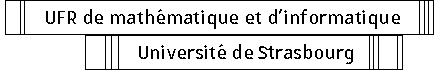
\includegraphics [width=8cm] {logo-ufr.pdf}       

    \vfill

    {
	\large
	\textsc{
	    Master d'informatique \\
	    Parcours I3D - IIRVIJ \\
		Imagerie 3D - Informatique Image Réalité Virtuelle Interaction et Jeux
	}
    }

    \bigskip\bigskip
    \bigskip\bigskip

    {\huge Rapport de projet}

    \bigskip\bigskip

    % Identité de l'auteur
    {\large Pierre \textsc{EVEN}}

    % Contact mail ou téléphone   
    {\small pierre.even@etu.unistra.fr}

    
    \vfill

    % Titre du TER : mettez un titre utile
    {
	\huge
	\textsc{
		Implémentation du jeu \\
	    ~ \\
        Pacman de 1980 en C++.
	}
    }

    \vfill
    \vfill

    \today

    \vfill

    {\large Projet réalisé avec}

    \medskip

    {
		\large Thomas \textsc{Torterotot} \small{thomas.torterotot@etu.unistra.fr}
	}

    \bigskip

    \bigskip
\end{center}

%%%%%%%%%%%%%%%%%%%%%%%%%%%%%%%%%%%%%%%%%%%%%%%%%%%%%%%%%%%%%%%%%%%%%%%%%%%%%%
% Table des matières
%%%%%%%%%%%%%%%%%%%%%%%%%%%%%%%%%%%%%%%%%%%%%%%%%%%%%%%%%%%%%%%%%%%%%%%%%%%%%%

{
    \parskip=0pt
    \tableofcontents
}
\begin{center}
    Historiquement, le jeu avait pour nom initial "PuckMan", nom qui sera par la suite changé \\
    en PacMan suite au passage de petits rigolos en ayant profité pour faire\\
    une mauvaise blague bien évidente.
    ~ \\
    Notre projet reprend ce nom original en hommage.
\end{center}

% Page blanche entre la table des matières et le texte
\cleardoublepage

%%%%%%%%%%%%%%%%%%%%%%%%%%%%%%%%%%%%%%%%%%%%%%%%%%%%%%%%%%%%%%%%%%%%%%%%%%%%%%
% Chapitre 1
%%%%%%%%%%%%%%%%%%%%%%%%%%%%%%%%%%%%%%%%%%%%%%%%%%%%%%%%%%%%%%%%%%%%%%%%%%%%%%

\chapter{État du projet}
    Le programme rendu reproduit plus ou moins fidèlement le comportement du jeu Pacman de 1980.
    Il est à noter que cette fidélité est suggestive, voici un résumé des fonctionnalités et
    différences avec le jeu original :
    \begin{itemize}
        \item Seul le gameplay principal a été reproduit, les menu et cinématiques ont été ignorés. 
        (par manque de temps, et le moteur n'est pas assez développé pour permettre l'implémentation
        rapide de ce genre de fonctionnalités)
        \item La gestion des coordonnées est gérée en interne sur des doubles, ce qui peut valoir des petits 
        écarts de comportement avec le jeu initial. Ce choix permet néanmoins un rendu plus fluide et est plus
        adapté aux pléthores de taux de rafraîchissement différents que l'on peut trouver sur un écran moderne.
        \item Les sprites et la map ne sont pas exactement ceux du jeu original (Ils correspondent à la version NES).
        Nous nous en sommes rendu compte tardivement ce qui nous a empêchés de les corriger. 
        Nous l'avons tout de même modifiée pour être plus pratique à utiliser.
        \item Aucun système de rendu de texte n'a encore été implémenté dans le moteur, c'est pourquoi il n'y a aucun
        texte visible dans le jeu. (les scores sont tout de même gérés et visibles dans la console)
        \item Manger une pac-gomme ou un fantôme ne ralentit / freeze pas le jeu contrairement au jeu original.
        Je trouve personnellement que c'est mieux comme ça car ça rend le jeu plus fluide.
        \item Le redimensionnement de la fenêtre est "en théorie" traité, mais il doit manquer quelques petits
        ajustements pour qu'il fonctionne sans bugs. C'est pourquoi il n'est pas disponible dans le programme fourni.
        (c'est un cas qui n'avait pas été prévu dans la conception initiale)
        \item Certains bugs du jeu original sont resimulés (ex sur l'IA des fantômes)
        \item L'algorithme de déplacement du joueur est le même que celui des fantômes, contrairement au jeu initial
        où le joueur est autorisé à "couper" les virages.
        \item Les fantômes ne sont pas ralentis dans le tunnel.
    \end{itemize}

    Pour le reste, tout suit plus ou moins fidèlement les algorithmes et comportements du jeu initial.
    (scores, vitesses, niveaux...)

\chapter{Implémentation et fonctionnement}
    Le programme est séparé en deux parties : le moteur et le jeu. Le moteur contient toute la partie utilitaire,
    rendu graphique et gestion de sprites. Celui-ci est conçu pour être
    réutilisable dans le contexte d'un autre jeu 2D utilisant des sprites simples. \\
    La partie jeu contient toutes les classes spécifiques au jeu PacMan.

    Les commentaires sont non-exhaustifs et concentrés dans les headers.
    Ils sont focalisés sur l'essentiel afin de faciliter la compréhension du programme par le relecteur.

\section{Le projet}
    L'architecture du projet se veut la plus standard possible selon les habitudes usuelles en C++.
    Les exécutables et binaires générés sont dans un dossier bin/, les assets du jeu sont dans resources/.
    Le programme doit être exécuté depuis la racine du projet. (le dossier resources doit se trouver à côté
    de l'exécutable)


\section{Le moteur}
    Le cœur du moteur passe par la classe \textit{Engine}. Celle-ci contient la gestion du delta-time, et du coeur de
    la boucle de rendu. (implémentée dans le main)
    Le moteur instancie une class \textit{Gamemode} qui contient toutes les informations relatives au jeu courant.

    C'est ce gamemode qui se chargera de créer le monde, les entités, gérer les scores etc...

    Le moteur inclut un système de gestion des sprites : \textit{sprite\_sheet.hpp}. Il est conçu pour être le plus
    intuitif et robuste possible pour l'utilisateur. Son implémentation est un peu plus complexe : les sprites sont
    manipulés via des \textit{SpriteHandles} (voir commentaires dans le header correspondant)

    Une classe template Vector2 a été implémentée pour représenter les coordonnées flottantes et discrètes, de même
    qu'une classe permettant de gérer facilement la notion de "direction".

    Aucune librairie externe n'a été utilisée mis à pars SDL, et éventuellement quelques classes utilitaires 
    comme logger.hpp, format.hpp et event\_manager.hpp. J'avais créé ces classes précédemment pour d'autres projets,
    et je les réutilise régulièrement. Elles ont été adaptées pour correspondre aux prérequis de ce projet.

\section{Le jeu}
    \begin{itemize}
        \item Le niveau est généré à partir d'un fichier texte (resources/level.map).
        Dans certain cas, un type de mur spécial "\^" et "v" doit être spécifié pour éviter à l'algorithme
        de génération relier des murs proches.
        \item La class Entity contient les informations de positionnement sur le terrain.
        \item La class Character hérite de Entity gère les déplacements des entitées sur le terrain, ainsi que la vitesse.
        \item GhostBase et Player héritent de Character et gèrent respectivement l'IA et le comportement des fantômes, et 
        la classe du joueur. (Les inputs sont restés dans le main par simplification)
        \item Initialement, nous pensions que les fantômes utilisaient un pathfinding avancé, c'est pour cette raison que nous
        en avons implémenté un dans la class pathfinding.hpp. Cependant en regardant plus précisément en détail le jeu original,
        il s'avère que celui-ci est beaucoup plus basique. Cette classe reste donc dans le projet comme relique mais n'est pas utilisée.
        \item Les différentes spécialisations de chaque type de fantôme sont implémentées dans ghosts.hpp (chacun hérite de GhostBase)
        \item PacmanGamemode contient tout le reste du gameplay. (le chargement des sprite est séparé dans un fichier à part : sprite\_loader.hpp)
    \end{itemize}

\section{Contribution individuelle}

    Dans ce projet, j'ai concentré mes efforts sur la base du moteur (Engine.cpp) ainsi qu'une grande partie du gameplay.
    J'ai essayé d'implémenter "rapidement" le gameplay le plus fidèlement possible au jeu original, et Thomas a pu repasser derrière moi
    pour corriger mes erreurs et oublis. Thomas s'est également chargé de la gestion du terrain. (chargement, cellules etc...)

    Note : Je pratique courament le C++ et le développement de moteurs de jeux depuis plusieurs années maintenant.
    Avec l'habitude j'arrive à être plutôt efficace : j'ai déjà implémenté de nombreuses fonctionnalités
    présentes dans ce projet à plusieurs reprises. Pour ces raisons la quantité de travail semblera peut être déséquilibrée, mais en 
    temps passé nous sommes à peu près sur le même ordre de grandeur.


\chapter{Limites et problèmes connus}

    Le moteur créé à l'occasion est très basique. Avec un peu plus de temps nous aurions pu implémenté un système d'affichage
    de texte pour les points. De même la gestion des timers est un peu "sale" actuellement et pourrait être déléguée à une 
    classe spécialisée dans le moteur.
    Il n'y a pas non plus de possibilité de charger un autre niveau ou de changer de gamemode.
    
    Pour ces raisons, implémenter les menus et les cinématiques aurait été très fastidieux sans ces outils.
    Au vu de la charge de travail et du temps déjà passé sur ce projet nous avons jugé que ce serait superflu et
    n'aurait pas servi à démontrer davantage nos compétences en C++ moderne.

\section{Bugs}
    A l'heure actuelle (où j'écris ce rapport) il reste quelques bugs mineurs à notre connaissance. En voici une liste exhaustive :

    \begin{itemize}
         \item Les fantômes se décalent parfois visuellement et ne sont pas tout à fait alignés avec les cases.
         \item Parfois (très rarement) un fantôme reste bloqué dans le spawn.
         \item Thomas a mentionné un bug où PacMan passait au-dessus du fruit ou d'un pac-gomme sans le manger, mais je n'ai pas pu reproduire le bug.
    \end{itemize}
\section{Conclusion}

    Ce projet était plutôt intéressant et motivant. Étant habitué travailler sur des moteurs 3D plus ou moins gros, en ayant eu l'occasion d'en
    implémenter une petite dizaine au cours de mon cursus, j'ai pu perfectionner mes techniques.
    Ce projet est donc plus une routine sans grande surprise pour moi mais toujours très fun. 
    (peut être un peu long quand même)

\section{Suggestions}

    Ayant un emploi du temps déjà très chargé avec les nombreux projets tous très chronophages de ce semestre,
    je souhaite faire quelques suggestions qui pourront peut être servir aux prochaines promo afin de leur faire gagner
    un peu de temps inutilement perdu, et réduire le facteur de stresse et d'inconnu :
    
    \begin{itemize}
        \item Le site "the pacman-dossier \url{https://pacman.holenet.info/} est une mine d'informations sur le jeu original.
        j'ai découvert son existence que très tardivement. Le mentionner dans le sujet aurait je pense été très pratique
        pour beaucoup d'entre nous.
        \item La sprite-map fournie correspond à celle du jeu Nes (et non pas le PacMan originel de 1980)
        \item Les attentes ne sont toujours pas très claires.
        Peut être que fournir une liste plus détaillée des fonctionnalités voulues aurait été plus simple à gérer pour nous
        que seulement demander de "reproduire" le jeu à l'identique. (avec éventuellement un bonus par suplément)
    \end{itemize}
    En espérant que ce retour vous aura été utile.
\end{document}
